Let $O$ be an optimal set and recall that we assume that $f(O) = 1$.
Let $T = \arg\max\{S, \displaystyle{\arg\max_{e \in U}}f(\{e\})\}$ 
be the set returned by the modified greedy algorithm, 
where $S$ is the set computed by the greedy algorithm~\ref{alg:greedy},
we prove the following theorem:

\begin{theorem}
$f(T) \geq (1 - e^{-1/2})$.
\end{theorem}

\begin{proof}
\end{proof}

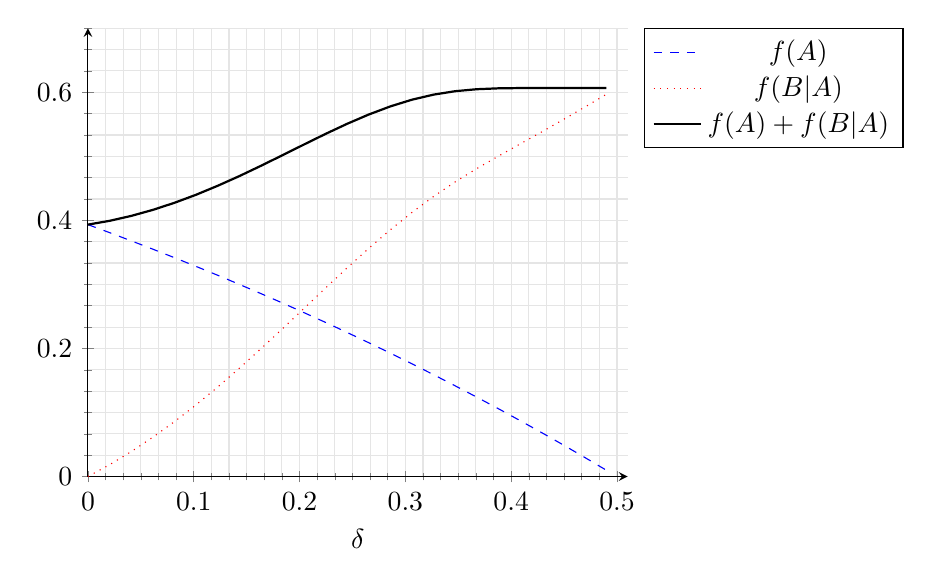
\begin{tikzpicture}
\begin{axis}[
	domain=0:0.49
	,ymax=.7
	,xmax=.51
	,xlabel=$\delta$
	,axis lines=left
	,grid=both
	,grid style={
		draw=gray!20
	}
	,minor tick num=5
	,legend pos=outer north east
	,legend entries={
		$f(A)$
		,$f(B|A)$
		,$f(A) + f(B|A)$
	}
]
  \addplot[blue, dashed, thin]{1-exp(-(0.5-x))};
  \addplot[red, dotted, thin]{(1 - exp(-(4*x/(1-2*x)))) * (exp(-1/2) - 1 + exp(-(1/2-x)))};
  \addplot[black, thick]{1-exp(-(0.5-x)) + (1 - exp(-(4*x/(1-2*x)))) * (exp(-1/2) - 1 + exp(-(1/2-x)))};
\end{axis}
\end{tikzpicture}

We denote by $x$ and $y$ the first two elements in $O$ dropped by the algorithm.  
We denote by $A$ the set of elements constructed by the algorithm just before
dropping $x$ and by $B$ the set of elements chosen by the algorithm right after dropping $x$ 
and just before dropping $y$.

\begin{figure}[h]
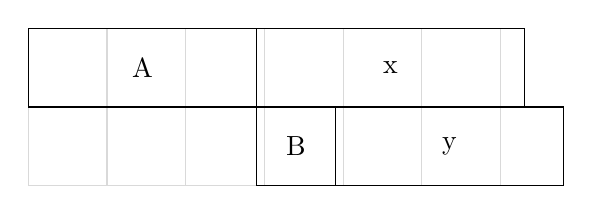
\begin{tikzpicture}[]
\draw[thin, gray!30] (0,-1) grid (6,1);
\draw 
	(0,1) 
	rectangle ++(2.9,-1) node[pos=.5]{A}
 	rectangle ++(1,-1) node[pos=.5]{B}
 	rectangle ++(2.9,+1) node[pos=.5]{y};
\draw (2.9, 0) rectangle +(3.4,1) node[pos=.5]{x};
	
\end{tikzpicture} 
\end{figure}

Let $c(A) = 1/2 - \delta$ 
then $c(x) > 1/2 + \delta$, $c(y) \leq 1/2 - \delta$, and $c(B) \geq 2\delta$.

\begin{lemma}
Let $S$ be any set and $C$ be the set produced by the algorithm 
before dropping the first element from $S$ then $f(C) \geq (1 - e^{-\frac{c(C)}{c(S)}})f(S)$.  
\end{lemma} 

\begin{observation}
$f(A) \geq (1 - e^{\delta - 1/2})f(O)$
\end{observation}

TODO verify this $\Downarrow$
\begin{observation}
$f_A(B) \geq (1 - e^{4\delta / (2\delta - 1)})f_A(O \setminus x)$
\end{observation}

\begin{observation}
$f(O \setminus x) \geq e^{-1/2}f(O)$
\end{observation}

Let $G$ be the set produced by the algorithm, then:
\begin{proof}
\def\arraystretch{1.5}
$$
\begin{array}{lll}
% 
f(G) & \geq f(A) + f_A(B)
\\& \geq f(A) + (1 - e^{4\delta / (2\delta - 1)})f_A(O \setminus x)
\\& = f(A) + (1 - e^{4\delta / (2\delta - 1)})(f(A \cup S \setminus x) - f(A))
\\& = e^{4\delta / (2\delta - 1)}f(A) 
	+ (1 - e^{4\delta / (2\delta - 1)})f(A \cup S \setminus x)
\\& \geq e^{4\delta / (2\delta - 1)}(1 - e^{\delta - 1/2})f(O)
	+ (1 - e^{4\delta / (2\delta - 1)})e^{-1/2}f(O)
\\& = [
		e^{4\delta / (2\delta - 1)}(1 - e^{\delta - 1/2}) + (1 - e^{4\delta / (2\delta - 1)})e^{-1/2}
		]f(O)
\\&& \geq (1-e^{-1/2})f(O)
% 
\end{array}
$$
\end{proof}